\documentclass{article}
\usepackage[mathcal,mathbf]{euler}
\usepackage{theorem,amsmath,enumerate,fancyhdr,amssymb,amsfonts}
\usepackage[pdftex]{graphics}
\usepackage{graphicx}

\usepackage{myDefs}

\title{ 
    Algorithmic Learning Theory\\
    Spring 2017\\
    Lecture 1
}
\author{
    {\bf Instructor:} Farid Alizadeh\\
    {\bf Scribe:} Yuan Qu
}
\date{01/18/2017} 

\begin{document}

\pagestyle{fancy}
\lhead{
    {\bf scribe:}Yuan Qu\\
    {\bf Lecture 1} 
} 
\rhead{
    {\bf Date: } 01/18/2017
} 

\maketitle

\medskip

There are 4 section in the Lecture 1:
\begin{enumerate}{
    \item Overview
    \item Fundamental Concepts
    \item Distinction of Concepts
    \item Bayesian Decision Rule  
}
\end{enumerate}
%% Write a quick short paragraph summarizing the topic covered in
%% the lecture here. You may use itemization or enumeration

\section{Overview}{
    Brief of the Syllabus and the tools needed.
    \subsection{Textbooks}{
        See \textit{Syllabus} in \textit{Sakai}.
    }
    \subsection{Student Work}{
        See \textit{Syllabus} in \textit{Sakai}.\\
        No test, \textbf{BUT}:
        \begin{enumerate}{
            \item Course note, in LaTeX
            \item Student projects (Can be in small group)  
        }
        \end{enumerate}
    }
    \subsection{Topics}{
        See \textit{Syllabus} in \textit{Sakai}.
    }
    \subsection{Tools}{
        \textit{R} \& \textit{RStudio}
    }
}

\section{Fundamental Concepts}{
    Introduction of basic concepts and ideas of machine learning.
    \subsection{Black Box}{
        \paragraph{Definition by Wikipedia:}{
            \textit{In science, computing, and engineering, a black box is a device, system or object which can be viewed in terms of its inputs and outputs (or transfer characteristics), without any knowledge of its internal workings.}\\
        }
        
        Consider a black box with a bunch of input and output,

        \begin{center}{
            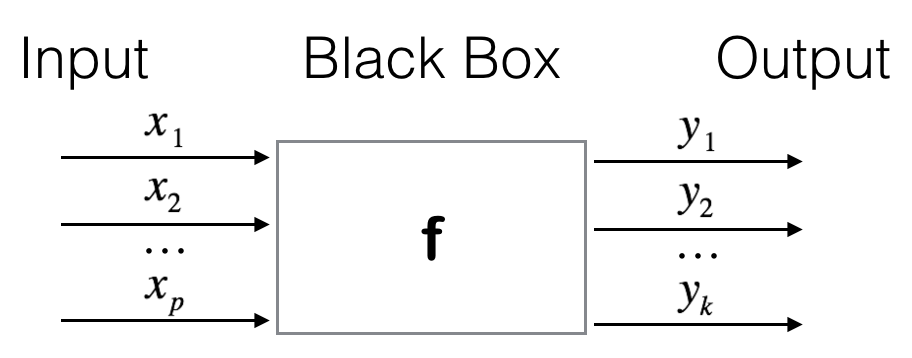
\includegraphics[scale=0.5]{blackbox.png}
        }
        \end{center}

        Which consists of 3 parts, Input, Output and the Function $f$:
        
        \paragraph{Input}{
            $x_1,x_2,...,x_p$, also called independ vars, predicators, features and controls.\\
            The input can be numerical or non-numerical(categorical), if input is in multi-class, it can be ordered(ordinal) or unordered.
        }

        \paragraph{Output}{
            $y_1,y_2,...,y_k$, also called response, depend vars and target vars. For example,

            \begin{center}{
                \begin{tabular}{|c|c|}
                \hline
                $f()$ & Output\\
                \hline
                regression & numerical \\
                \hline
                classification & categorical \\
                \hline
                \end{tabular}
            }
            \end{center}   
        }
    }
    \subsection{Data}{
        \paragraph{Definition by Wikipedia: Data(computing)}{
            \textit{is any sequence of one or more symbols given meaning by specific act(s) of interpretation.\\
        }
        
        Data is also called example and observation and usually organized by table, like this:

        \begin{center}{
            \begin{tabular}{|c|c|c|c|c|c|c|c|c|}
            \hline
            row & $x_1$ & $x_2$ & ... & $x_p$ & $y_1$ & $y_2$ & ... & $y_k$\\
            \hline
            1 & ... & ... & ... & ... & ... & ... & ... & ... \\
            \hline
            2 & ... & ... & ... & ... & ... & ... & ... & ... \\
            \hline
            ... & ... & ... & ... & ... & ... & ... & ... & ... \\
            \hline
            N & ... & ... & ... & ... & ... & ... & ... & ... \\
            \hline
            \end{tabular}
        }
        \end{center} 

        The data table can be regarded as \(\hat{f}\), an estimation of $f$, which is considered an algorithm or a rule.\\
        For most application scenarios, data is given or generated by an algorithm called generation method.\\
        In a dataset, there may be some missing data(N/A) in the table.\\
    }

    \subsection{Big Data}{
        Data that can't be located in one computer.
        \paragraph{"Big"}{
            large scale in 2 dimensions, the number of records/items(rows) and the number of features(columns).
        }
        \paragraph{More features is good?}{
            There may be some irrelevant or redundant features in dataset, so that feature selection is a major problem.
        }
    }   
}
\section{Distinctions}{
    The distinctions between some concepts in machine learning.
    \subsection{Parametric vs Non-parametric}{
        \paragraph{e.g.}{
            \(x = height, y = weight, y = f(x)\)
        }
        \subsubsection{Parametric}{
            e.g. Regression\\
            Assumption: $y = b_0 + b_1 x$, $b_0, b_1$ are the parameters.\\
            So, the problem can be showed like this:

            \begin{center}{
                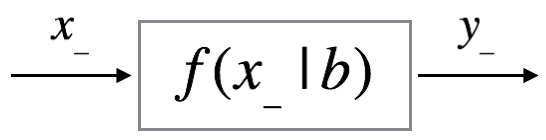
\includegraphics[scale=0.5]{f(x_|b).png}
            }
            \end{center}

            The work of machine learning is to get data and find the parameters.\\

            Supposed we get the dataset like this:

            \begin{center}{
                \begin{tabular}{|c|c|}
                \hline
                $W$ & $H$ \\
                \hline
                $w_1$ & $h_1$ \\
                \hline
                $w_2$ & $h_2$ \\
                \hline
                ... & ... \\
                \hline
                $w_n$ & $h_n$ \\
                \hline
                \end{tabular}
            }
            \end{center} 

            Assume: $w = b_0 + b_1 h$\\
            So, the regression plot is: \(\hat{w}=\hat{b_0}+\hat{b_1} h\)

            % \begin{center}{
            %     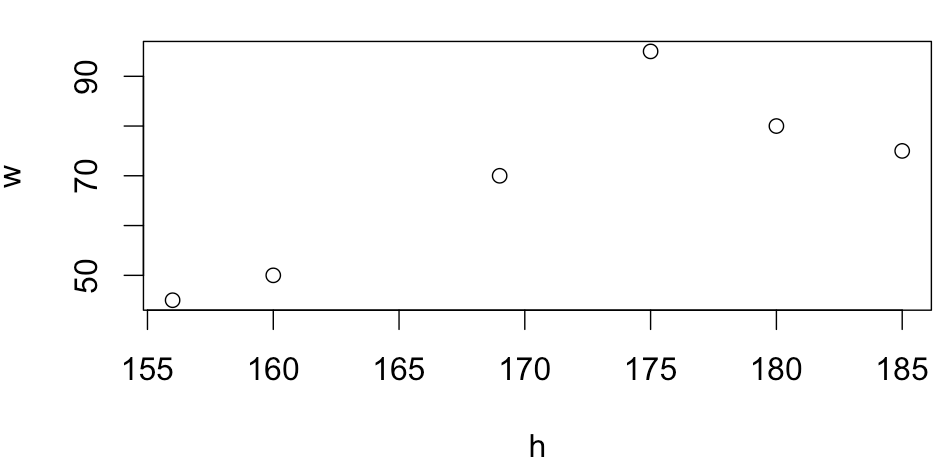
\includegraphics[scale=0.5]{plot(m).png}
            % }
            % \end{center}

            \begin{center}{
                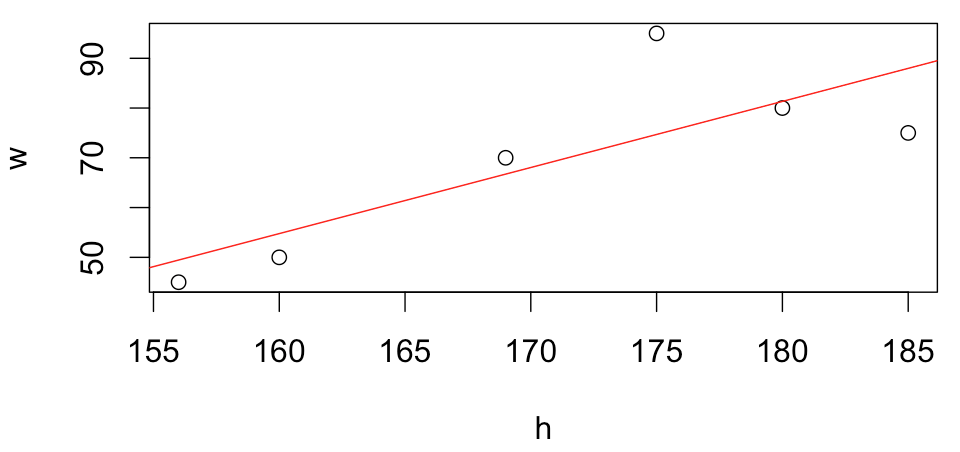
\includegraphics[scale=0.5]{regression.png}
            }
            \end{center}
        }
        \subsubsection{Non-parametric}{
            e.g. kNN.(k-nearest neighbors algorithm)\\

            if $k=3$, find $k$ near point of $h_{new}$, so,\\
            \begin{center}{
                \(w_{new}=\)average(k closest points to \(h_{new}\))\(=\frac{w_1+w_2+w_3}{3}\)
            }
            \end{center}

            \begin{center}{
                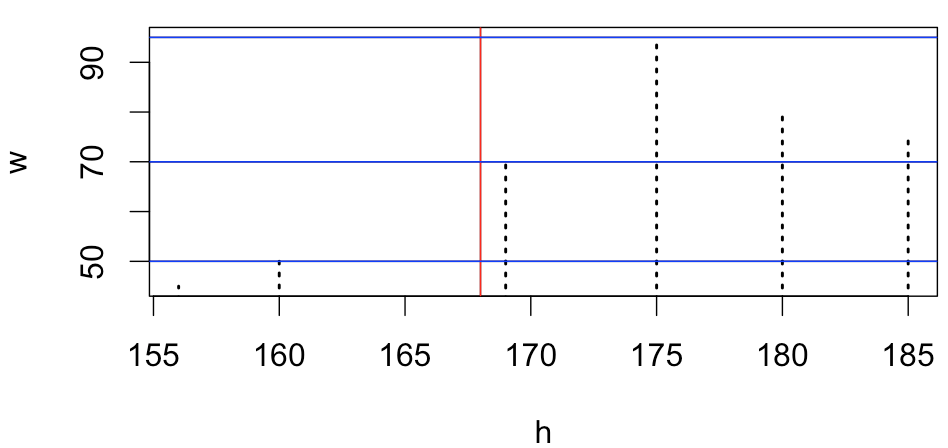
\includegraphics[scale=0.5]{knn.png}
            }
            \end{center}

            In this case, the $h_{new}$ is the red line, so, the $w_1, w_2, w_3$ are the $w$ in blue lines.      
        }
        \subsubsection{Conclusion}{
            \paragraph{Parametric}{
                Assumption: $y = b_0 + b_1 x$, $b_0, b_1$ are the parameters.\\
                \begin{center}{
                    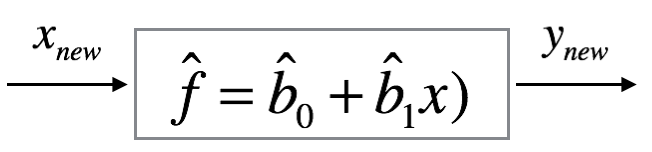
\includegraphics[scale=0.5]{parametric.png}
                }
                \end{center}
            }
            \paragraph{Non-parametric}{
                More flexible. No parameters to impose, no assumption. 
            }
        }
    }
    \subsection{Supervised vs Unsupervised(non-supervised)}{
        \paragraph{Supervised}{
            Name $x$ and $y$, the input and output are specific by labels.
        }
        \paragraph{Unsupervised}{
            Every column of data is $x$, no labels.\\
            e.g $k$-means
            \begin{center}{
                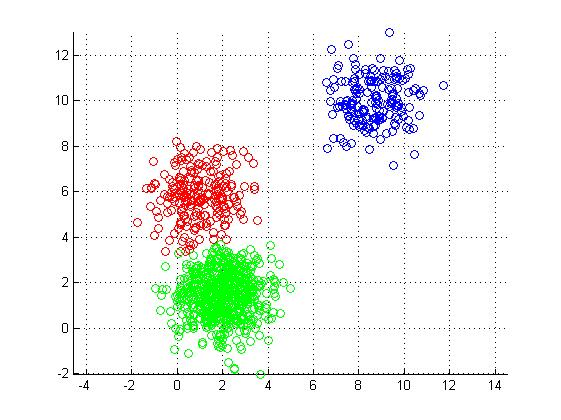
\includegraphics[scale=0.5]{k-means.jpg}
            }
            \end{center}
            When the number of dimensions increase, the difficulty of recognition increase, so that the selection of $x$ is a major problem.
        }
    }
    \subsection{Online learning vs Offline(not online) learning}{
        \paragraph{Online learning}{
            data becomes available in a sequential order and is used to update our best predictor for future data at each step.
        }
        \paragraph{Offline(not online) learning}{
            generate the best predictor by learning on the entire training data set at once.
        }
    }
    \subsection{Loss vs Overfitting}{
        \subsubsection{Loss for classification}{
            \paragraph{Definition by Wikipedia}{
                a loss function or cost function is a function that maps an event or values of one or more variables onto a real number intuitively representing some "cost" associated with the event.
            }

            \begin{center}{
                
                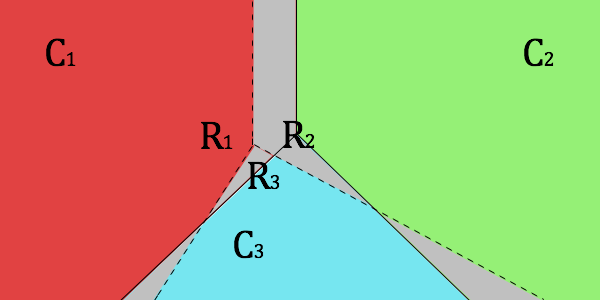
\includegraphics{classification.png}
            }
            \end{center}

            The true classification is $f$, and the classes are $C_1, C_2,$ and $C_3$, which are divided by line and painted in red, green and blue. Supposed that we don't know the true classification.\\
            The estimated classification is \(\hat{f}\), and the classes are $R_1, R_2,$ and $R_3$, divided by dotted line.\\
            The mistake area, painted by gray, is the difference between estimation and true classification.\\
            Loss function abstract the size of mistake area.\\

            \begin{center}{
                \(P_x(t) \to \) Probability density function
            }
            \end{center}

            Misclassification rate: \[Pr_x[f(x)\not=\hat{f}(x)]\]
            But misclassification rate above is not computable, because we have to know two function or classification.\\

            Empirical error/misclassification rate: \[\frac{Number\;of\;misclassified\;data}{Total\;data\;number}\]

            \paragraph{Loss matrix}{
                To show the cost of error in a matrix.
                \begin{center}{
                    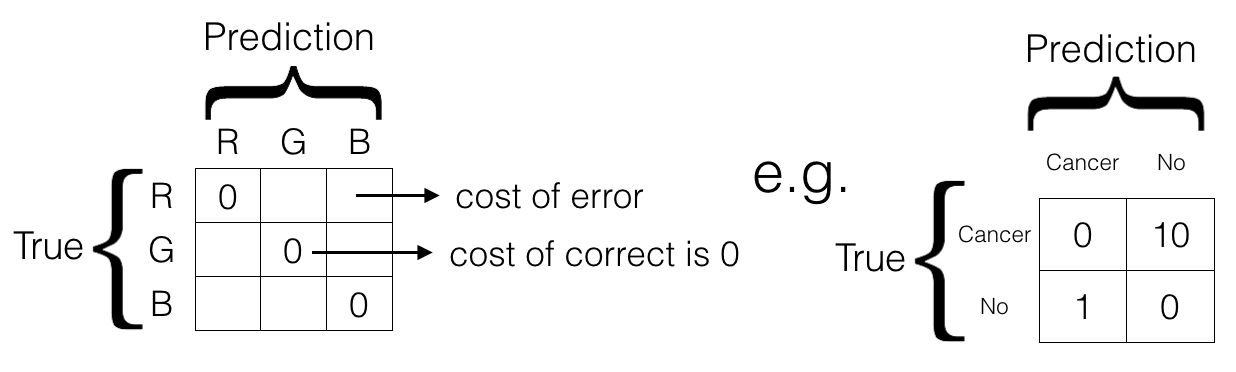
\includegraphics[scale=0.5]{lossmatrix.png}
                }
                \end{center}
            }

        }
        \subsubsection{Loss for regression}{
            \begin{center}{
                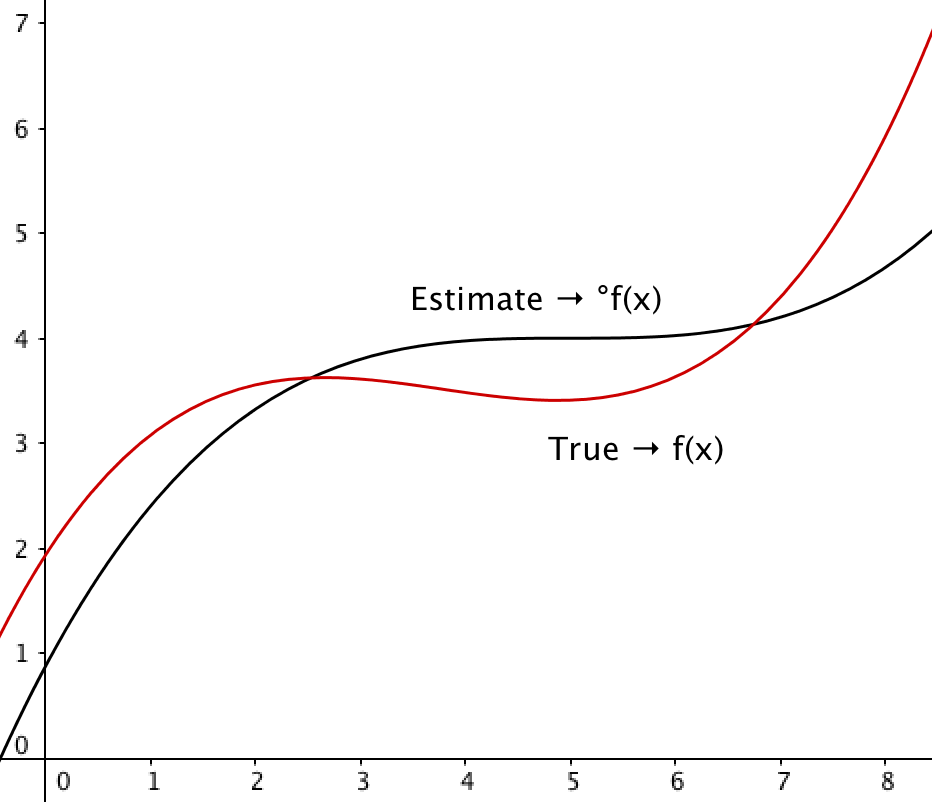
\includegraphics[scale=0.5]{loss-regression.png}
            }
            \end{center}
             Mean square error is used to eliminate the + and -.\\
             Loss function: \(E_x\big(\ell(f,\hat{f},x)\big)\)\\
             Error rate: \[\int\ell(f,\hat{f},x)p(x)dx=\int\big(f(x)-\hat{f}(x)\big)^2p(x)dx\]
             Major of loss: \(Max{|f(x)-\hat{f}(x)|}\)\\
             Empirical error: \[\frac{\sum_{i=1}^{N}\big(f(x)-\hat{f}(x)\big)^2}{N}\]
        }
        \subsubsection{Overfitting}{    
            \paragraph{Definition by Wikipedia}{
                In overfitting, a statistical model describes random error or noise instead of the underlying relationship. Overfitting occurs when a model is excessively complex, such as having too many parameters relative to the number of observations.
            }

            In this case, overfitting is that the $\hat{f}(x)$ performs in perfect result. Generally, overfitting is a bad phenomenon, because the data self may have error or miss relevant vars.

            \paragraph{Validation set}{
                The technique to guard overfitting from complex model.\\
                \begin{enumerate}{
                    \item Set a set of data aside(validation set)
                    \item learning is done on the remaining data(training set)
                    \item Use validation set to predict response
                }
                \end{enumerate}
            }
        }
    }
}

\section{Bayesian Decision Rule}{
    \paragraph{Bayes Law:}{
        For Event $A$ and Event $B$
        \[0 \le P[A] \le 1, 0 \le P[B] \le 1 \]

        \begin{center}{
            ($A$ and $B$: $A \cap B$, $A$ or $B$: $A \cup B$, not $A$: $\bar{A}$ or $A^*$)
        }
        \end{center}

        \begin{center}{
            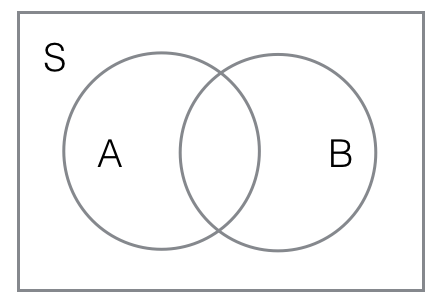
\includegraphics[scale=0.5]{bayes.png}
        }
        \end{center}

        If,
        \begin{equation}
            A \cap B \neq \emptyset, 
        \end{equation}
        
        So, according to (1),
        \begin{equation}
            P[A|B]= \frac{P[A \cap B]}{P[B]} \Rightarrow P[A \cap B] = P[A|B] \times P[B],
        \end{equation}

        And, the same with (2),
        \begin{equation}
            P[B|A]= \frac{P[B \cap A]}{P[A]} \Rightarrow P[B \cap A] = P[B|A] \times P[A]
        \end{equation}

        Obviously, we have,
        \begin{equation}
            P[A|B]P[B] = P[B|A]P[A]
        \end{equation}

        So,  
        \[P[A|B] = \frac{P[B|A] \times P[A]}{P[B]}\]
        \[P[B|A] = \frac{P[A|B] \times P[B]}{P[A]}\]

        \paragraph{e.g.}{
            If, a partition of $A$,
            \begin{center}{
                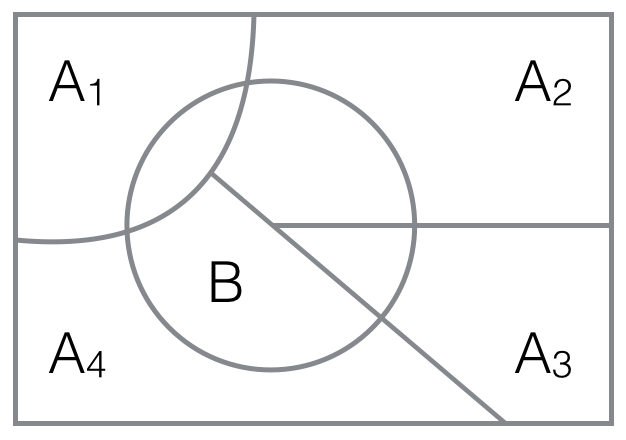
\includegraphics[scale=0.5]{bayes-eg.png}
            }
            \end{center}

            \[A_1 \cup A_2 \cup A_3 \cup A_4 = S, A_i \cap A_j = \emptyset, i,j=1,2,3,4\]
            So,
            \[P[B] = \sum_{i=1}^{4}P[B|A_i]P[A_i]\]
        }

    }
}

%give a one paragraph short description of the topics


% Add additional sections and sub section as need with appropriate
% titles
% section{  }

%\subsection{ }
%\subsubsection{ }

%% For including graphs or pictures use a .pdf pr .png type pictures
%% format and use the follwoing to include it in your file. Note
%% that scale isuse tp resize the graph if it is too big or too
%% small:

%\begin{center}
%\includegraphics[scale=0.5]{filename.pdf}
%\end{center

\end{document}